\documentclass[10pt,a4paper]{article}
\usepackage[T1]{fontenc}
\usepackage[margin=22mm]{geometry}
\usepackage{amsmath,amssymb,amsthm,booktabs,array,longtable,graphicx,url,microtype}
\usepackage[hidelinks]{hyperref}
\usepackage{fancyhdr}
\pagestyle{fancy}\fancyhf{}\fancyhead[L]{Supplementary Material}\fancyfoot[C]{\thepage}
\setlength{\headheight}{13pt}
\renewcommand{\thesection}{S\arabic{section}}
\renewcommand{\thetable}{S\arabic{table}}
\renewcommand{\thefigure}{S\arabic{figure}}
\newcommand{\BA}{\operatorname{BA}}
\makeatletter\newcommand{\tableinput}[1]{\@@input #1.tex }\makeatother
\begin{document}
\begin{center}
{\Large\bfseries Supplementary Material}\par\medskip
{\large Model Selection for Energy-Aware Edge Intrusion Detection: A Controlled Measurement Study}\par\medskip
Nuonan Ouyang, Adrian Shatte, Zhigang Lu, Chao Chen, and Wei Xiang
\end{center}

\section{Reading the Results}\label{sec:guide}
Sections S2--S7 give details of the six-method physical comparison reported in the paper. Each of ten blocks contains one 500-second workload per method, with a fresh 60-second preceding idle. The block is the unit of paired inference. The methods share the workload within a block and the fixed detector pool.

Additional classifier and fixed-rate software experiments are presented separately in Sections S8--S9. Their state definitions, workloads, and policy-selection procedures differ from the physical comparison; their observations are not combined with the ten-block estimates. This distinction is particularly important for training curves and reward-weight sensitivity, which describe the specified fixed-rate objective rather than the physical study's service-penalized objective.

\section{Controller Configuration}\label{sec:configuration}
The deployed action order is TinyDT, LightLR, MedRF, HeavyMLP. The common observation contains current arrivals, FIFO carryover before current arrivals are appended, previous mean selected-path score, and previous action. The three numerical coordinates have three bins each and previous action has four values, giving 108 states. All models use binary threshold 0.5. No policy is updated during deployment.

\begin{table}[h!]\centering\small
\caption{Policy-training parameters for the physical comparison.}
\begin{tabular}{p{.39\linewidth}p{.52\linewidth}}\toprule
Parameter & Value\\\midrule
Episodes and windows per episode & 1,000 and 500\\
Training seeds & 2003, 2011, 2017, 2027, 2029\\
Exploration & Linear, 1.0 to 0.01 across episodes\\
Discount & 0.9\\
Q-learning rate and initialization & 0.1; zero Q table\\
Tie breaking & First maximizing action in the configured order\\
DQN network & One-hot 108 inputs; 64/64 ReLU hidden units; 4 outputs\\
DQN optimizer and loss & Adam, learning rate 0.001; Smooth-L1 loss\\
Replay and minibatch & Capacity 10,000; warm-up 320; minibatch 32\\
Target network & Hard update every 250 optimizer steps\\
Gradient norm & Clipped at 10\\
Eligible checkpoint & Last episode only\\
Seed selection & Maximum summed validation reward; smallest seed breaks a tie\\
Selected policies & Q seed 2011; DQN seed 2003\\\bottomrule
\end{tabular}\end{table}

Twenty-five policies are trained: five full Q policies, five full DQN policies, and five Q policies for each of three coordinate removals (arrival, threat, previous action). Each has 500,000 recorded transitions. The full-state policies selected for deployment each visit 36 encoded states in training. The physical comparison reaches 12 states for each selected learned policy; every one occurs in the corresponding training record. This is support coverage, not proof of optimal behavior throughout the 108-state space. The training simulator never produces nonzero carryover, and temperature is not an action-attributable reward component.

The physical controller loads the recorded policy weights and uses the common count-based observation. Some configuration files retain descriptive fields from the earlier five-coordinate scheduler; the execution entry point uses the 108-state encoder specified here. Reproduction should use the supplied runtime entry point rather than infer execution from unused descriptive fields.

\section{Information and Computation}\label{sec:information}
\begin{table}[h!]\centering\small
\caption{Information available to the deployed methods.}
\begin{tabular}{p{.23\linewidth}p{.33\linewidth}p{.34\linewidth}}\toprule
Method & Before window inference & During inference\\\midrule
Static-LightLR / Static-MedRF & Fixed action & Selected model scores\\
Q / DQN & Arrival, pre-arrival backlog, prior threat, prior action & Selected model scores; no online updates\\
DeadlineGuard & Current work count and fixed MedRF batch p95 & Selected model scores\\
Cascade & Fixed LightLR entry path & Current LightLR scores; MedRF scores on the uncertain subset\\\bottomrule
\end{tabular}\end{table}

Cascade evaluates LightLR on the full batch. The uncertainty mask is inclusive at both 0.3 and 0.7. If any row is deferred, MedRF is called once on that subset; otherwise MedRF is not called. The final vector combines LightLR and deferred MedRF scores in the original row order. This is sub-batch inference, not one forest call per uncertain row. The mean completed score becomes the next window's context, and the common previous-action field records the LightLR entry action for Cascade.

No deployed method sees ground-truth labels, future-window arrival counts, true current prevalence, or cached counterfactual detector scores. Offline training uses labels and model-score caches to construct its reward. The cascade's use of current confidence follows paid entry inference and is not a claim that it receives the same information as pre-window RL.

\section{Utility and Reward Interpretation}\label{sec:utility}
For immediate utility $U_a(s)=w_DD_a(s)-C_a(s)$, define
\[
g_{ab}(s)=D_a(s)-D_b(s)-[C_a(s)-C_b(s)]/w_D.
\]
For $w_D>0$, the sign of $U_a-U_b$ is the sign of $g_{ab}$. A strict pairwise reversal exists exactly when two attainable states have margins of opposite signs. On finite support this is equivalent to $\min g_{ab}<0<\max g_{ab}$. A zero margin is a tie. On nonfinite support the existence formulation avoids assuming extrema are attained.

With state-independent costs, the implied threshold is $\tau_{ab}=(C_a-C_b)/w_D$. With state-dependent completion and pending-work costs, the threshold itself depends on state and must remain inside $g_{ab}(s)$. A third detector can dominate both members of a reversing pair. Long-horizon values also contain future-state terms. Neither the pairwise algebra nor a sampled action map proves that a learned policy must be constant or globally optimal.

For a min--max power term, $\Delta C_P=w_P(P_a-P_b)/(P_{\max}-P_{\min})$. Its denominator depends on the candidate pool. A budget-based denominator has a direct physical interpretation, but changing it would define another objective. We retain the measured policies and do not present such a change as an observed improvement.

\section{Timing, Interruptions, and Analysis Sets}\label{sec:timing}
The meter supplies boundary-inclusive samples at nominal 1 Hz. Voltage and signed current are decoded from the original frames; the recorded orientation is used consistently to obtain positive consumed power. The integration times are request/receive midpoints, and adjacent samples are combined by the trapezoidal rule. Average power is energy divided by the observed integration duration, not automatically by 500.

Preceding idle retains the instrumented runtime and detector residency but performs no detector inference. Adjusted energy is $E-\bar P_{\mathrm{idle}}\Delta\tau$, and adjusted mean power is $E/\Delta\tau-\bar P_{\mathrm{idle}}$. Negative adjusted values are possible when a workload mean is below its preceding idle; they are not negative physical consumption.

Two attempts fail the fixed monitoring conditions. In block 1, the Static-LightLR workload stops after an external-CPU trigger. Its later workload uses a newly collected idle and replaces the failed workload. In block 5, Cascade's preceding idle stops on a sampling-interval trigger before the formal workload begins; a new idle is followed by the first completed workload for that position. Failed attempts are excluded; accepted portions of each block are retained. Both blocks consequently span separated measurement periods.

The CPU calculation brackets allowed worker-process counters with global CPU counters and conservatively includes unattributed kernel and transient work in external activity. The ceiling is 5\% and the interval limit is 1.5 s. Before the block-5 recovery, sample-relative waiting replaces an additional one-second wait after processing, and rejected-interval snapshots are retained. The ceiling, interval limit, policies, and service logic stay unchanged. The earlier failed interval lacks the rejected right snapshot, so its exact duration cannot be recovered.

Set A contains all ten complete blocks. Set B excludes block 1 ($n=9$, df=8); set C excludes blocks 1 and 5 ($n=8$, df=7). Set A uses df=9. Recovery sensitivities were added during execution; the complete method-pair enumeration was recorded later. They are additional analyses, not original preregistered endpoints. All sets and raw/adjusted outcomes are reported. Their agreement cannot establish complete removal of temporal drift or instrumentation effects.

\section{Run-Level Results}\label{sec:runs}
The following table gives all accepted workloads. Order is the actual within-block position. Raw and preceding-idle-adjusted energies are in joules. The original full-precision values are available in the repository. Every listed workload completes 627,500 rows, with zero recorded late-completed rows, window deadline misses, and final backlog.
\small\setlength{\tabcolsep}{5pt}\begin{longtable}{rrlrrrr}
\caption{All accepted workloads.}\label{tab:runs}\\
\toprule Block & Order & Method & Raw (J) & Adjusted (J) & F1 & Recall (\%)\\\midrule\endfirsthead
\toprule Block & Order & Method & Raw (J) & Adjusted (J) & F1 & Recall (\%)\\\midrule\endhead
\bottomrule\endfoot
1 & 1 & DQN & 1430.1 & 1.5 & 0.9763 & 96.677\\
1 & 2 & Cascade & 1478.8 & 50.7 & 0.9902 & 99.417\\
1 & 3 & Static-MedRF & 1493.9 & 63.9 & 0.9907 & 99.660\\
1 & 4 & Q-learning & 1431.6 & -12.9 & 0.9763 & 96.677\\
1 & 5 & DeadlineGuard & 1482.2 & 58.3 & 0.9907 & 99.660\\
1 & 6 & Static-LightLR & 1433.6 & 10.8 & 0.9763 & 96.677\\
2 & 1 & DeadlineGuard & 1486.1 & 54.5 & 0.9906 & 99.629\\
2 & 2 & DQN & 1430.8 & -2.7 & 0.9764 & 96.685\\
2 & 3 & Static-MedRF & 1482.3 & 54.0 & 0.9906 & 99.629\\
2 & 4 & Static-LightLR & 1427.3 & -9.4 & 0.9764 & 96.685\\
2 & 5 & Cascade & 1466.5 & 41.6 & 0.9901 & 99.391\\
2 & 6 & Q-learning & 1429.9 & -1.1 & 0.9764 & 96.685\\
3 & 1 & Cascade & 1470.0 & 55.2 & 0.9902 & 99.397\\
3 & 2 & Q-learning & 1429.8 & -0.3 & 0.9763 & 96.666\\
3 & 3 & Static-LightLR & 1427.5 & -3.3 & 0.9763 & 96.666\\
3 & 4 & Static-MedRF & 1480.6 & 40.0 & 0.9906 & 99.633\\
3 & 5 & DQN & 1433.1 & 6.0 & 0.9763 & 96.666\\
3 & 6 & DeadlineGuard & 1477.7 & 59.2 & 0.9906 & 99.633\\
4 & 1 & Static-MedRF & 1480.9 & 45.8 & 0.9904 & 99.630\\
4 & 2 & DeadlineGuard & 1481.6 & 56.3 & 0.9904 & 99.630\\
4 & 3 & Q-learning & 1444.9 & 9.6 & 0.9760 & 96.632\\
4 & 4 & Cascade & 1484.4 & 33.2 & 0.9900 & 99.384\\
4 & 5 & DQN & 1443.8 & 6.8 & 0.9760 & 96.632\\
4 & 6 & Static-LightLR & 1442.3 & 16.3 & 0.9760 & 96.632\\
5 & 1 & Static-LightLR & 1452.1 & 23.3 & 0.9762 & 96.650\\
5 & 2 & Q-learning & 1438.6 & -13.7 & 0.9762 & 96.650\\
5 & 3 & DeadlineGuard & 1495.8 & 54.8 & 0.9906 & 99.646\\
5 & 4 & DQN & 1442.5 & 12.2 & 0.9762 & 96.650\\
5 & 5 & Static-MedRF & 1504.4 & 70.7 & 0.9906 & 99.646\\
5 & 6 & Cascade & 1489.8 & 41.9 & 0.9901 & 99.398\\
6 & 1 & DeadlineGuard & 1497.5 & 57.7 & 0.9908 & 99.659\\
6 & 2 & Static-MedRF & 1503.7 & 50.8 & 0.9908 & 99.659\\
6 & 3 & Cascade & 1487.1 & 37.2 & 0.9904 & 99.419\\
6 & 4 & Q-learning & 1455.0 & 23.1 & 0.9767 & 96.724\\
6 & 5 & Static-LightLR & 1454.3 & 18.2 & 0.9767 & 96.724\\
6 & 6 & DQN & 1449.4 & -6.4 & 0.9767 & 96.724\\
7 & 1 & Cascade & 1484.3 & 29.1 & 0.9900 & 99.392\\
7 & 2 & DQN & 1454.9 & 10.1 & 0.9760 & 96.639\\
7 & 3 & Q-learning & 1454.3 & 16.3 & 0.9760 & 96.639\\
7 & 4 & Static-LightLR & 1445.1 & -5.3 & 0.9760 & 96.639\\
7 & 5 & DeadlineGuard & 1509.8 & 62.9 & 0.9905 & 99.638\\
7 & 6 & Static-MedRF & 1503.4 & 64.5 & 0.9905 & 99.638\\
8 & 1 & Q-learning & 1446.1 & -0.9 & 0.9765 & 96.730\\
8 & 2 & Cascade & 1495.8 & 38.9 & 0.9903 & 99.433\\
8 & 3 & DeadlineGuard & 1506.6 & 59.7 & 0.9906 & 99.669\\
8 & 4 & DQN & 1445.7 & 9.6 & 0.9765 & 96.730\\
8 & 5 & Static-LightLR & 1449.1 & -5.4 & 0.9765 & 96.730\\
8 & 6 & Static-MedRF & 1504.9 & 51.9 & 0.9906 & 99.669\\
9 & 1 & Q-learning & 1439.4 & 3.5 & 0.9765 & 96.707\\
9 & 2 & Static-MedRF & 1484.6 & 63.8 & 0.9907 & 99.656\\
9 & 3 & Cascade & 1473.6 & 27.7 & 0.9903 & 99.417\\
9 & 4 & DeadlineGuard & 1488.7 & 56.1 & 0.9907 & 99.656\\
9 & 5 & Static-LightLR & 1434.3 & 8.2 & 0.9765 & 96.707\\
9 & 6 & DQN & 1431.1 & 4.2 & 0.9765 & 96.707\\
10 & 1 & Static-MedRF & 1487.5 & 53.1 & 0.9906 & 99.671\\
10 & 2 & Static-LightLR & 1434.2 & -2.6 & 0.9763 & 96.695\\
10 & 3 & DQN & 1444.4 & 19.3 & 0.9763 & 96.695\\
10 & 4 & Cascade & 1475.4 & 42.1 & 0.9902 & 99.429\\
10 & 5 & Q-learning & 1432.5 & -20.8 & 0.9763 & 96.695\\
10 & 6 & DeadlineGuard & 1495.1 & 70.0 & 0.9906 & 99.671\\
\end{longtable}\normalsize


\section{Complete Paired Comparisons}\label{sec:paired}
Each difference is the first method minus the second within a block. C denotes Cascade, DG DeadlineGuard, LR Static-LightLR, RF Static-MedRF, and Q Tabular-Q. Energy is in J and power in W. F1, recall, FPR, and balanced-accuracy differences are expressed in percentage points. Counts retain their row or window units. SD is the sample standard deviation of block differences.

The intervals are nominal Student-$t$ 95\% intervals, without multiplicity correction. An interval spanning zero does not establish equivalence. All methods have the same completed-row count and zero recorded late rows, final backlog, and deadline-miss windows; their corresponding pairwise differences, SDs, and formula-based intervals are zero. Such zero intervals summarize the observed constant differences and are not guarantees of future service reliability.
\footnotesize\setlength{\tabcolsep}{4pt}\begin{longtable}{lllrrr}
\caption{All 540 method-pair, metric, and analysis-set combinations.}\label{tab:allpairs}\\
\toprule Pair & Outcome & Set & Mean & SD & 95\% CI\\\midrule\endfirsthead
\toprule Pair & Outcome & Set & Mean & SD & 95\% CI\\\midrule\endhead
\bottomrule\endfoot
LR--Q & Energy (J) & A & -0.25 & 6.01 & $[-4.55,4.05]$\\
LR--Q & Energy (J) & B & -0.49 & 6.32 & $[-5.35,4.37]$\\
LR--Q & Energy (J) & C & -2.23 & 3.79 & $[-5.40,0.93]$\\
LR--Q & Power (W) & A & -0.0005 & 0.0120 & $[-0.0091,0.0081]$\\
LR--Q & Power (W) & B & -0.0010 & 0.0126 & $[-0.0107,0.0087]$\\
LR--Q & Power (W) & C & -0.0045 & 0.0076 & $[-0.0108,0.0018]$\\
LR--Q & Adjusted energy (J) & A & 4.79 & 17.27 & $[-7.56,17.15]$\\
LR--Q & Adjusted energy (J) & B & 2.69 & 16.91 & $[-10.31,15.69]$\\
LR--Q & Adjusted energy (J) & C & -1.59 & 11.74 & $[-11.41,8.22]$\\
LR--Q & Adjusted power (W) & A & 0.0096 & 0.0345 & $[-0.0151,0.0343]$\\
LR--Q & Adjusted power (W) & B & 0.0054 & 0.0338 & $[-0.0206,0.0314]$\\
LR--Q & Adjusted power (W) & C & -0.0032 & 0.0235 & $[-0.0228,0.0164]$\\
LR--Q & F1 (pp) & A & 0.0000 & 0.0000 & $[0.0000,0.0000]$\\
LR--Q & F1 (pp) & B & 0.0000 & 0.0000 & $[0.0000,0.0000]$\\
LR--Q & F1 (pp) & C & 0.0000 & 0.0000 & $[0.0000,0.0000]$\\
LR--Q & Recall (pp) & A & 0.0000 & 0.0000 & $[0.0000,0.0000]$\\
LR--Q & Recall (pp) & B & 0.0000 & 0.0000 & $[0.0000,0.0000]$\\
LR--Q & Recall (pp) & C & 0.0000 & 0.0000 & $[0.0000,0.0000]$\\
LR--Q & FPR (pp) & A & 0.0000 & 0.0000 & $[0.0000,0.0000]$\\
LR--Q & FPR (pp) & B & 0.0000 & 0.0000 & $[0.0000,0.0000]$\\
LR--Q & FPR (pp) & C & 0.0000 & 0.0000 & $[0.0000,0.0000]$\\
LR--Q & BA (pp) & A & 0.0000 & 0.0000 & $[0.0000,0.0000]$\\
LR--Q & BA (pp) & B & 0.0000 & 0.0000 & $[0.0000,0.0000]$\\
LR--Q & BA (pp) & C & 0.0000 & 0.0000 & $[0.0000,0.0000]$\\
LR--Q & Missed windows & A & 0 & 0 & $[0,0]$\\
LR--Q & Missed windows & B & 0 & 0 & $[0,0]$\\
LR--Q & Missed windows & C & 0 & 0 & $[0,0]$\\
LR--Q & Late rows & A & 0 & 0 & $[0,0]$\\
LR--Q & Late rows & B & 0 & 0 & $[0,0]$\\
LR--Q & Late rows & C & 0 & 0 & $[0,0]$\\
LR--Q & Completed rows & A & 0 & 0 & $[0,0]$\\
LR--Q & Completed rows & B & 0 & 0 & $[0,0]$\\
LR--Q & Completed rows & C & 0 & 0 & $[0,0]$\\
LR--Q & Final backlog & A & 0 & 0 & $[0,0]$\\
LR--Q & Final backlog & B & 0 & 0 & $[0,0]$\\
LR--Q & Final backlog & C & 0 & 0 & $[0,0]$\\
LR--DQN & Energy (J) & A & -0.60 & 6.60 & $[-5.32,4.12]$\\
LR--DQN & Energy (J) & B & -1.05 & 6.83 & $[-6.30,4.21]$\\
LR--DQN & Energy (J) & C & -2.38 & 5.93 & $[-7.33,2.58]$\\
LR--DQN & Power (W) & A & -0.0012 & 0.0132 & $[-0.0106,0.0082]$\\
LR--DQN & Power (W) & B & -0.0021 & 0.0136 & $[-0.0126,0.0084]$\\
LR--DQN & Power (W) & C & -0.0048 & 0.0118 & $[-0.0147,0.0051]$\\
LR--DQN & Adjusted energy (J) & A & -0.97 & 14.88 & $[-11.62,9.67]$\\
LR--DQN & Adjusted energy (J) & B & -2.12 & 15.31 & $[-13.88,9.65]$\\
LR--DQN & Adjusted energy (J) & C & -3.77 & 15.47 & $[-16.71,9.16]$\\
LR--DQN & Adjusted power (W) & A & -0.0019 & 0.0298 & $[-0.0232,0.0193]$\\
LR--DQN & Adjusted power (W) & B & -0.0042 & 0.0306 & $[-0.0278,0.0193]$\\
LR--DQN & Adjusted power (W) & C & -0.0076 & 0.0309 & $[-0.0334,0.0183]$\\
LR--DQN & F1 (pp) & A & 0.0000 & 0.0000 & $[0.0000,0.0000]$\\
LR--DQN & F1 (pp) & B & 0.0000 & 0.0000 & $[0.0000,0.0000]$\\
LR--DQN & F1 (pp) & C & 0.0000 & 0.0000 & $[0.0000,0.0000]$\\
LR--DQN & Recall (pp) & A & 0.0000 & 0.0000 & $[0.0000,0.0000]$\\
LR--DQN & Recall (pp) & B & 0.0000 & 0.0000 & $[0.0000,0.0000]$\\
LR--DQN & Recall (pp) & C & 0.0000 & 0.0000 & $[0.0000,0.0000]$\\
LR--DQN & FPR (pp) & A & 0.0000 & 0.0000 & $[0.0000,0.0000]$\\
LR--DQN & FPR (pp) & B & 0.0000 & 0.0000 & $[0.0000,0.0000]$\\
LR--DQN & FPR (pp) & C & 0.0000 & 0.0000 & $[0.0000,0.0000]$\\
LR--DQN & BA (pp) & A & 0.0000 & 0.0000 & $[0.0000,0.0000]$\\
LR--DQN & BA (pp) & B & 0.0000 & 0.0000 & $[0.0000,0.0000]$\\
LR--DQN & BA (pp) & C & 0.0000 & 0.0000 & $[0.0000,0.0000]$\\
LR--DQN & Missed windows & A & 0 & 0 & $[0,0]$\\
LR--DQN & Missed windows & B & 0 & 0 & $[0,0]$\\
LR--DQN & Missed windows & C & 0 & 0 & $[0,0]$\\
LR--DQN & Late rows & A & 0 & 0 & $[0,0]$\\
LR--DQN & Late rows & B & 0 & 0 & $[0,0]$\\
LR--DQN & Late rows & C & 0 & 0 & $[0,0]$\\
LR--DQN & Completed rows & A & 0 & 0 & $[0,0]$\\
LR--DQN & Completed rows & B & 0 & 0 & $[0,0]$\\
LR--DQN & Completed rows & C & 0 & 0 & $[0,0]$\\
LR--DQN & Final backlog & A & 0 & 0 & $[0,0]$\\
LR--DQN & Final backlog & B & 0 & 0 & $[0,0]$\\
LR--DQN & Final backlog & C & 0 & 0 & $[0,0]$\\
LR--C & Energy (J) & A & -40.60 & 3.95 & $[-43.42,-37.77]$\\
LR--C & Energy (J) & B & -40.09 & 3.82 & $[-43.03,-37.15]$\\
LR--C & Energy (J) & C & -40.38 & 3.98 & $[-43.71,-37.06]$\\
LR--C & Power (W) & A & -0.0812 & 0.0079 & $[-0.0869,-0.0756]$\\
LR--C & Power (W) & B & -0.0802 & 0.0076 & $[-0.0861,-0.0743]$\\
LR--C & Power (W) & C & -0.0808 & 0.0079 & $[-0.0874,-0.0741]$\\
LR--C & Adjusted energy (J) & A & -34.68 & 15.29 & $[-45.61,-23.74]$\\
LR--C & Adjusted energy (J) & B & -34.09 & 16.10 & $[-46.47,-21.72]$\\
LR--C & Adjusted energy (J) & C & -36.03 & 16.05 & $[-49.45,-22.61]$\\
LR--C & Adjusted power (W) & A & -0.0694 & 0.0306 & $[-0.0912,-0.0475]$\\
LR--C & Adjusted power (W) & B & -0.0682 & 0.0322 & $[-0.0929,-0.0434]$\\
LR--C & Adjusted power (W) & C & -0.0721 & 0.0321 & $[-0.0989,-0.0452]$\\
LR--C & F1 (pp) & A & -1.3843 & 0.0105 & $[-1.3918,-1.3768]$\\
LR--C & F1 (pp) & B & -1.3838 & 0.0110 & $[-1.3922,-1.3753]$\\
LR--C & F1 (pp) & C & -1.3829 & 0.0114 & $[-1.3925,-1.3734]$\\
LR--C & Recall (pp) & A & -2.7274 & 0.0219 & $[-2.7431,-2.7118]$\\
LR--C & Recall (pp) & B & -2.7259 & 0.0227 & $[-2.7434,-2.7085]$\\
LR--C & Recall (pp) & C & -2.7232 & 0.0226 & $[-2.7421,-2.7043]$\\
LR--C & FPR (pp) & A & -0.0127 & 0.0056 & $[-0.0167,-0.0087]$\\
LR--C & FPR (pp) & B & -0.0122 & 0.0057 & $[-0.0165,-0.0078]$\\
LR--C & FPR (pp) & C & -0.0109 & 0.0046 & $[-0.0147,-0.0071]$\\
LR--C & BA (pp) & A & -1.3574 & 0.0100 & $[-1.3645,-1.3502]$\\
LR--C & BA (pp) & B & -1.3569 & 0.0105 & $[-1.3649,-1.3488]$\\
LR--C & BA (pp) & C & -1.3561 & 0.0109 & $[-1.3653,-1.3470]$\\
LR--C & Missed windows & A & 0 & 0 & $[0,0]$\\
LR--C & Missed windows & B & 0 & 0 & $[0,0]$\\
LR--C & Missed windows & C & 0 & 0 & $[0,0]$\\
LR--C & Late rows & A & 0 & 0 & $[0,0]$\\
LR--C & Late rows & B & 0 & 0 & $[0,0]$\\
LR--C & Late rows & C & 0 & 0 & $[0,0]$\\
LR--C & Completed rows & A & 0 & 0 & $[0,0]$\\
LR--C & Completed rows & B & 0 & 0 & $[0,0]$\\
LR--C & Completed rows & C & 0 & 0 & $[0,0]$\\
LR--C & Final backlog & A & 0 & 0 & $[0,0]$\\
LR--C & Final backlog & B & 0 & 0 & $[0,0]$\\
LR--C & Final backlog & C & 0 & 0 & $[0,0]$\\
LR--DG & Energy (J) & A & -52.14 & 8.46 & $[-58.20,-46.09]$\\
LR--DG & Energy (J) & B & -52.53 & 8.88 & $[-59.36,-45.70]$\\
LR--DG & Energy (J) & C & -53.63 & 8.81 & $[-61.00,-46.27]$\\
LR--DG & Power (W) & A & -0.1043 & 0.0169 & $[-0.1164,-0.0922]$\\
LR--DG & Power (W) & B & -0.1051 & 0.0178 & $[-0.1187,-0.0914]$\\
LR--DG & Power (W) & C & -0.1073 & 0.0176 & $[-0.1220,-0.0925]$\\
LR--DG & Adjusted energy (J) & A & -53.86 & 14.28 & $[-64.08,-43.64]$\\
LR--DG & Adjusted energy (J) & B & -54.56 & 14.97 & $[-66.07,-43.05]$\\
LR--DG & Adjusted energy (J) & C & -57.45 & 13.05 & $[-68.36,-46.54]$\\
LR--DG & Adjusted power (W) & A & -0.1077 & 0.0286 & $[-0.1282,-0.0873]$\\
LR--DG & Adjusted power (W) & B & -0.1091 & 0.0299 & $[-0.1321,-0.0861]$\\
LR--DG & Adjusted power (W) & C & -0.1149 & 0.0261 & $[-0.1367,-0.0931]$\\
LR--DG & F1 (pp) & A & -1.4288 & 0.0131 & $[-1.4382,-1.4195]$\\
LR--DG & F1 (pp) & B & -1.4277 & 0.0133 & $[-1.4379,-1.4174]$\\
LR--DG & F1 (pp) & C & -1.4263 & 0.0136 & $[-1.4377,-1.4149]$\\
LR--DG & Recall (pp) & A & -2.9686 & 0.0254 & $[-2.9868,-2.9504]$\\
LR--DG & Recall (pp) & B & -2.9669 & 0.0264 & $[-2.9873,-2.9466]$\\
LR--DG & Recall (pp) & C & -2.9633 & 0.0257 & $[-2.9848,-2.9418]$\\
LR--DG & FPR (pp) & A & -0.1660 & 0.0077 & $[-0.1716,-0.1605]$\\
LR--DG & FPR (pp) & B & -0.1668 & 0.0078 & $[-0.1728,-0.1608]$\\
LR--DG & FPR (pp) & C & -0.1657 & 0.0075 & $[-0.1720,-0.1594]$\\
LR--DG & BA (pp) & A & -1.4013 & 0.0126 & $[-1.4103,-1.3922]$\\
LR--DG & BA (pp) & B & -1.4001 & 0.0128 & $[-1.4099,-1.3902]$\\
LR--DG & BA (pp) & C & -1.3988 & 0.0131 & $[-1.4097,-1.3879]$\\
LR--DG & Missed windows & A & 0 & 0 & $[0,0]$\\
LR--DG & Missed windows & B & 0 & 0 & $[0,0]$\\
LR--DG & Missed windows & C & 0 & 0 & $[0,0]$\\
LR--DG & Late rows & A & 0 & 0 & $[0,0]$\\
LR--DG & Late rows & B & 0 & 0 & $[0,0]$\\
LR--DG & Late rows & C & 0 & 0 & $[0,0]$\\
LR--DG & Completed rows & A & 0 & 0 & $[0,0]$\\
LR--DG & Completed rows & B & 0 & 0 & $[0,0]$\\
LR--DG & Completed rows & C & 0 & 0 & $[0,0]$\\
LR--DG & Final backlog & A & 0 & 0 & $[0,0]$\\
LR--DG & Final backlog & B & 0 & 0 & $[0,0]$\\
LR--DG & Final backlog & C & 0 & 0 & $[0,0]$\\
LR--RF & Energy (J) & A & -52.66 & 5.96 & $[-56.92,-48.40]$\\
LR--RF & Energy (J) & B & -51.80 & 5.63 & $[-56.13,-47.48]$\\
LR--RF & Energy (J) & C & -51.74 & 6.01 & $[-56.77,-46.71]$\\
LR--RF & Power (W) & A & -0.1053 & 0.0119 & $[-0.1138,-0.0968]$\\
LR--RF & Power (W) & B & -0.1036 & 0.0112 & $[-0.1122,-0.0950]$\\
LR--RF & Power (W) & C & -0.1035 & 0.0120 & $[-0.1135,-0.0934]$\\
LR--RF & Adjusted energy (J) & A & -50.77 & 12.76 & $[-59.89,-41.64]$\\
LR--RF & Adjusted energy (J) & B & -50.50 & 13.51 & $[-60.89,-40.12]$\\
LR--RF & Adjusted energy (J) & C & -50.89 & 14.39 & $[-62.92,-38.86]$\\
LR--RF & Adjusted power (W) & A & -0.1015 & 0.0255 & $[-0.1198,-0.0833]$\\
LR--RF & Adjusted power (W) & B & -0.1010 & 0.0270 & $[-0.1218,-0.0802]$\\
LR--RF & Adjusted power (W) & C & -0.1018 & 0.0288 & $[-0.1258,-0.0777]$\\
LR--RF & F1 (pp) & A & -1.4288 & 0.0131 & $[-1.4382,-1.4195]$\\
LR--RF & F1 (pp) & B & -1.4277 & 0.0133 & $[-1.4379,-1.4174]$\\
LR--RF & F1 (pp) & C & -1.4263 & 0.0136 & $[-1.4377,-1.4149]$\\
LR--RF & Recall (pp) & A & -2.9686 & 0.0254 & $[-2.9868,-2.9504]$\\
LR--RF & Recall (pp) & B & -2.9669 & 0.0264 & $[-2.9873,-2.9466]$\\
LR--RF & Recall (pp) & C & -2.9633 & 0.0257 & $[-2.9848,-2.9418]$\\
LR--RF & FPR (pp) & A & -0.1660 & 0.0077 & $[-0.1716,-0.1605]$\\
LR--RF & FPR (pp) & B & -0.1668 & 0.0078 & $[-0.1728,-0.1608]$\\
LR--RF & FPR (pp) & C & -0.1657 & 0.0075 & $[-0.1720,-0.1594]$\\
LR--RF & BA (pp) & A & -1.4013 & 0.0126 & $[-1.4103,-1.3922]$\\
LR--RF & BA (pp) & B & -1.4001 & 0.0128 & $[-1.4099,-1.3902]$\\
LR--RF & BA (pp) & C & -1.3988 & 0.0131 & $[-1.4097,-1.3879]$\\
LR--RF & Missed windows & A & 0 & 0 & $[0,0]$\\
LR--RF & Missed windows & B & 0 & 0 & $[0,0]$\\
LR--RF & Missed windows & C & 0 & 0 & $[0,0]$\\
LR--RF & Late rows & A & 0 & 0 & $[0,0]$\\
LR--RF & Late rows & B & 0 & 0 & $[0,0]$\\
LR--RF & Late rows & C & 0 & 0 & $[0,0]$\\
LR--RF & Completed rows & A & 0 & 0 & $[0,0]$\\
LR--RF & Completed rows & B & 0 & 0 & $[0,0]$\\
LR--RF & Completed rows & C & 0 & 0 & $[0,0]$\\
LR--RF & Final backlog & A & 0 & 0 & $[0,0]$\\
LR--RF & Final backlog & B & 0 & 0 & $[0,0]$\\
LR--RF & Final backlog & C & 0 & 0 & $[0,0]$\\
Q--DQN & Energy (J) & A & -0.35 & 5.48 & $[-4.28,3.57]$\\
Q--DQN & Energy (J) & B & -0.56 & 5.78 & $[-5.00,3.88]$\\
Q--DQN & Energy (J) & C & -0.14 & 6.03 & $[-5.18,4.90]$\\
Q--DQN & Power (W) & A & -0.0007 & 0.0109 & $[-0.0086,0.0071]$\\
Q--DQN & Power (W) & B & -0.0011 & 0.0115 & $[-0.0100,0.0077]$\\
Q--DQN & Power (W) & C & -0.0003 & 0.0120 & $[-0.0104,0.0098]$\\
Q--DQN & Adjusted energy (J) & A & -5.77 & 18.92 & $[-19.30,7.77]$\\
Q--DQN & Adjusted energy (J) & B & -4.81 & 19.81 & $[-20.04,10.42]$\\
Q--DQN & Adjusted energy (J) & C & -2.18 & 19.43 & $[-18.43,14.06]$\\
Q--DQN & Adjusted power (W) & A & -0.0115 & 0.0378 & $[-0.0386,0.0155]$\\
Q--DQN & Adjusted power (W) & B & -0.0096 & 0.0396 & $[-0.0401,0.0208]$\\
Q--DQN & Adjusted power (W) & C & -0.0044 & 0.0389 & $[-0.0369,0.0281]$\\
Q--DQN & F1 (pp) & A & 0.0000 & 0.0000 & $[0.0000,0.0000]$\\
Q--DQN & F1 (pp) & B & 0.0000 & 0.0000 & $[0.0000,0.0000]$\\
Q--DQN & F1 (pp) & C & 0.0000 & 0.0000 & $[0.0000,0.0000]$\\
Q--DQN & Recall (pp) & A & 0.0000 & 0.0000 & $[0.0000,0.0000]$\\
Q--DQN & Recall (pp) & B & 0.0000 & 0.0000 & $[0.0000,0.0000]$\\
Q--DQN & Recall (pp) & C & 0.0000 & 0.0000 & $[0.0000,0.0000]$\\
Q--DQN & FPR (pp) & A & 0.0000 & 0.0000 & $[0.0000,0.0000]$\\
Q--DQN & FPR (pp) & B & 0.0000 & 0.0000 & $[0.0000,0.0000]$\\
Q--DQN & FPR (pp) & C & 0.0000 & 0.0000 & $[0.0000,0.0000]$\\
Q--DQN & BA (pp) & A & 0.0000 & 0.0000 & $[0.0000,0.0000]$\\
Q--DQN & BA (pp) & B & 0.0000 & 0.0000 & $[0.0000,0.0000]$\\
Q--DQN & BA (pp) & C & 0.0000 & 0.0000 & $[0.0000,0.0000]$\\
Q--DQN & Missed windows & A & 0 & 0 & $[0,0]$\\
Q--DQN & Missed windows & B & 0 & 0 & $[0,0]$\\
Q--DQN & Missed windows & C & 0 & 0 & $[0,0]$\\
Q--DQN & Late rows & A & 0 & 0 & $[0,0]$\\
Q--DQN & Late rows & B & 0 & 0 & $[0,0]$\\
Q--DQN & Late rows & C & 0 & 0 & $[0,0]$\\
Q--DQN & Completed rows & A & 0 & 0 & $[0,0]$\\
Q--DQN & Completed rows & B & 0 & 0 & $[0,0]$\\
Q--DQN & Completed rows & C & 0 & 0 & $[0,0]$\\
Q--DQN & Final backlog & A & 0 & 0 & $[0,0]$\\
Q--DQN & Final backlog & B & 0 & 0 & $[0,0]$\\
Q--DQN & Final backlog & C & 0 & 0 & $[0,0]$\\
Q--C & Energy (J) & A & -40.35 & 7.34 & $[-45.60,-35.10]$\\
Q--C & Energy (J) & B & -39.60 & 7.37 & $[-45.26,-33.94]$\\
Q--C & Energy (J) & C & -38.15 & 6.35 & $[-43.46,-32.84]$\\
Q--C & Power (W) & A & -0.0807 & 0.0147 & $[-0.0912,-0.0702]$\\
Q--C & Power (W) & B & -0.0792 & 0.0147 & $[-0.0905,-0.0679]$\\
Q--C & Power (W) & C & -0.0763 & 0.0127 & $[-0.0869,-0.0657]$\\
Q--C & Adjusted energy (J) & A & -39.47 & 19.71 & $[-53.57,-25.37]$\\
Q--C & Adjusted energy (J) & B & -36.79 & 18.87 & $[-51.29,-22.28]$\\
Q--C & Adjusted energy (J) & C & -34.44 & 18.71 & $[-50.08,-18.79]$\\
Q--C & Adjusted power (W) & A & -0.0789 & 0.0394 & $[-0.1071,-0.0507]$\\
Q--C & Adjusted power (W) & B & -0.0736 & 0.0377 & $[-0.1026,-0.0446]$\\
Q--C & Adjusted power (W) & C & -0.0689 & 0.0374 & $[-0.1002,-0.0376]$\\
Q--C & F1 (pp) & A & -1.3843 & 0.0105 & $[-1.3918,-1.3768]$\\
Q--C & F1 (pp) & B & -1.3838 & 0.0110 & $[-1.3922,-1.3753]$\\
Q--C & F1 (pp) & C & -1.3829 & 0.0114 & $[-1.3925,-1.3734]$\\
Q--C & Recall (pp) & A & -2.7274 & 0.0219 & $[-2.7431,-2.7118]$\\
Q--C & Recall (pp) & B & -2.7259 & 0.0227 & $[-2.7434,-2.7085]$\\
Q--C & Recall (pp) & C & -2.7232 & 0.0226 & $[-2.7421,-2.7043]$\\
Q--C & FPR (pp) & A & -0.0127 & 0.0056 & $[-0.0167,-0.0087]$\\
Q--C & FPR (pp) & B & -0.0122 & 0.0057 & $[-0.0165,-0.0078]$\\
Q--C & FPR (pp) & C & -0.0109 & 0.0046 & $[-0.0147,-0.0071]$\\
Q--C & BA (pp) & A & -1.3574 & 0.0100 & $[-1.3645,-1.3502]$\\
Q--C & BA (pp) & B & -1.3569 & 0.0105 & $[-1.3649,-1.3488]$\\
Q--C & BA (pp) & C & -1.3561 & 0.0109 & $[-1.3653,-1.3470]$\\
Q--C & Missed windows & A & 0 & 0 & $[0,0]$\\
Q--C & Missed windows & B & 0 & 0 & $[0,0]$\\
Q--C & Missed windows & C & 0 & 0 & $[0,0]$\\
Q--C & Late rows & A & 0 & 0 & $[0,0]$\\
Q--C & Late rows & B & 0 & 0 & $[0,0]$\\
Q--C & Late rows & C & 0 & 0 & $[0,0]$\\
Q--C & Completed rows & A & 0 & 0 & $[0,0]$\\
Q--C & Completed rows & B & 0 & 0 & $[0,0]$\\
Q--C & Completed rows & C & 0 & 0 & $[0,0]$\\
Q--C & Final backlog & A & 0 & 0 & $[0,0]$\\
Q--C & Final backlog & B & 0 & 0 & $[0,0]$\\
Q--C & Final backlog & C & 0 & 0 & $[0,0]$\\
Q--DG & Energy (J) & A & -51.90 & 8.11 & $[-57.70,-46.10]$\\
Q--DG & Energy (J) & B & -52.04 & 8.59 & $[-58.64,-45.44]$\\
Q--DG & Energy (J) & C & -51.40 & 8.95 & $[-58.88,-43.91]$\\
Q--DG & Power (W) & A & -0.1038 & 0.0162 & $[-0.1154,-0.0922]$\\
Q--DG & Power (W) & B & -0.1041 & 0.0172 & $[-0.1173,-0.0909]$\\
Q--DG & Power (W) & C & -0.1028 & 0.0179 & $[-0.1178,-0.0878]$\\
Q--DG & Adjusted energy (J) & A & -58.65 & 15.67 & $[-69.86,-47.44]$\\
Q--DG & Adjusted energy (J) & B & -57.25 & 15.94 & $[-69.51,-45.00]$\\
Q--DG & Adjusted energy (J) & C & -55.86 & 16.44 & $[-69.60,-42.11]$\\
Q--DG & Adjusted power (W) & A & -0.1173 & 0.0313 & $[-0.1397,-0.0949]$\\
Q--DG & Adjusted power (W) & B & -0.1145 & 0.0319 & $[-0.1390,-0.0900]$\\
Q--DG & Adjusted power (W) & C & -0.1117 & 0.0329 & $[-0.1392,-0.0842]$\\
Q--DG & F1 (pp) & A & -1.4288 & 0.0131 & $[-1.4382,-1.4195]$\\
Q--DG & F1 (pp) & B & -1.4277 & 0.0133 & $[-1.4379,-1.4174]$\\
Q--DG & F1 (pp) & C & -1.4263 & 0.0136 & $[-1.4377,-1.4149]$\\
Q--DG & Recall (pp) & A & -2.9686 & 0.0254 & $[-2.9868,-2.9504]$\\
Q--DG & Recall (pp) & B & -2.9669 & 0.0264 & $[-2.9873,-2.9466]$\\
Q--DG & Recall (pp) & C & -2.9633 & 0.0257 & $[-2.9848,-2.9418]$\\
Q--DG & FPR (pp) & A & -0.1660 & 0.0077 & $[-0.1716,-0.1605]$\\
Q--DG & FPR (pp) & B & -0.1668 & 0.0078 & $[-0.1728,-0.1608]$\\
Q--DG & FPR (pp) & C & -0.1657 & 0.0075 & $[-0.1720,-0.1594]$\\
Q--DG & BA (pp) & A & -1.4013 & 0.0126 & $[-1.4103,-1.3922]$\\
Q--DG & BA (pp) & B & -1.4001 & 0.0128 & $[-1.4099,-1.3902]$\\
Q--DG & BA (pp) & C & -1.3988 & 0.0131 & $[-1.4097,-1.3879]$\\
Q--DG & Missed windows & A & 0 & 0 & $[0,0]$\\
Q--DG & Missed windows & B & 0 & 0 & $[0,0]$\\
Q--DG & Missed windows & C & 0 & 0 & $[0,0]$\\
Q--DG & Late rows & A & 0 & 0 & $[0,0]$\\
Q--DG & Late rows & B & 0 & 0 & $[0,0]$\\
Q--DG & Late rows & C & 0 & 0 & $[0,0]$\\
Q--DG & Completed rows & A & 0 & 0 & $[0,0]$\\
Q--DG & Completed rows & B & 0 & 0 & $[0,0]$\\
Q--DG & Completed rows & C & 0 & 0 & $[0,0]$\\
Q--DG & Final backlog & A & 0 & 0 & $[0,0]$\\
Q--DG & Final backlog & B & 0 & 0 & $[0,0]$\\
Q--DG & Final backlog & C & 0 & 0 & $[0,0]$\\
Q--RF & Energy (J) & A & -52.41 & 8.65 & $[-58.60,-46.23]$\\
Q--RF & Energy (J) & B & -51.31 & 8.40 & $[-57.77,-44.86]$\\
Q--RF & Energy (J) & C & -49.51 & 6.85 & $[-55.23,-43.78]$\\
Q--RF & Power (W) & A & -0.1048 & 0.0173 & $[-0.1172,-0.0924]$\\
Q--RF & Power (W) & B & -0.1026 & 0.0168 & $[-0.1155,-0.0897]$\\
Q--RF & Power (W) & C & -0.0990 & 0.0137 & $[-0.1104,-0.0876]$\\
Q--RF & Adjusted energy (J) & A & -55.56 & 18.53 & $[-68.81,-42.31]$\\
Q--RF & Adjusted energy (J) & B & -53.20 & 17.98 & $[-67.02,-39.37]$\\
Q--RF & Adjusted energy (J) & C & -49.30 & 14.60 & $[-61.50,-37.09]$\\
Q--RF & Adjusted power (W) & A & -0.1111 & 0.0371 & $[-0.1376,-0.0846]$\\
Q--RF & Adjusted power (W) & B & -0.1064 & 0.0360 & $[-0.1340,-0.0787]$\\
Q--RF & Adjusted power (W) & C & -0.0986 & 0.0292 & $[-0.1230,-0.0742]$\\
Q--RF & F1 (pp) & A & -1.4288 & 0.0131 & $[-1.4382,-1.4195]$\\
Q--RF & F1 (pp) & B & -1.4277 & 0.0133 & $[-1.4379,-1.4174]$\\
Q--RF & F1 (pp) & C & -1.4263 & 0.0136 & $[-1.4377,-1.4149]$\\
Q--RF & Recall (pp) & A & -2.9686 & 0.0254 & $[-2.9868,-2.9504]$\\
Q--RF & Recall (pp) & B & -2.9669 & 0.0264 & $[-2.9873,-2.9466]$\\
Q--RF & Recall (pp) & C & -2.9633 & 0.0257 & $[-2.9848,-2.9418]$\\
Q--RF & FPR (pp) & A & -0.1660 & 0.0077 & $[-0.1716,-0.1605]$\\
Q--RF & FPR (pp) & B & -0.1668 & 0.0078 & $[-0.1728,-0.1608]$\\
Q--RF & FPR (pp) & C & -0.1657 & 0.0075 & $[-0.1720,-0.1594]$\\
Q--RF & BA (pp) & A & -1.4013 & 0.0126 & $[-1.4103,-1.3922]$\\
Q--RF & BA (pp) & B & -1.4001 & 0.0128 & $[-1.4099,-1.3902]$\\
Q--RF & BA (pp) & C & -1.3988 & 0.0131 & $[-1.4097,-1.3879]$\\
Q--RF & Missed windows & A & 0 & 0 & $[0,0]$\\
Q--RF & Missed windows & B & 0 & 0 & $[0,0]$\\
Q--RF & Missed windows & C & 0 & 0 & $[0,0]$\\
Q--RF & Late rows & A & 0 & 0 & $[0,0]$\\
Q--RF & Late rows & B & 0 & 0 & $[0,0]$\\
Q--RF & Late rows & C & 0 & 0 & $[0,0]$\\
Q--RF & Completed rows & A & 0 & 0 & $[0,0]$\\
Q--RF & Completed rows & B & 0 & 0 & $[0,0]$\\
Q--RF & Completed rows & C & 0 & 0 & $[0,0]$\\
Q--RF & Final backlog & A & 0 & 0 & $[0,0]$\\
Q--RF & Final backlog & B & 0 & 0 & $[0,0]$\\
Q--RF & Final backlog & C & 0 & 0 & $[0,0]$\\
DQN--C & Energy (J) & A & -40.00 & 7.17 & $[-45.13,-34.87]$\\
DQN--C & Energy (J) & B & -39.04 & 6.90 & $[-44.34,-33.74]$\\
DQN--C & Energy (J) & C & -38.00 & 6.58 & $[-43.51,-32.50]$\\
DQN--C & Power (W) & A & -0.0800 & 0.0143 & $[-0.0902,-0.0697]$\\
DQN--C & Power (W) & B & -0.0781 & 0.0138 & $[-0.0887,-0.0675]$\\
DQN--C & Power (W) & C & -0.0760 & 0.0131 & $[-0.0870,-0.0650]$\\
DQN--C & Adjusted energy (J) & A & -33.70 & 11.62 & $[-42.02,-25.39]$\\
DQN--C & Adjusted energy (J) & B & -31.98 & 10.88 & $[-40.34,-23.61]$\\
DQN--C & Adjusted energy (J) & C & -32.25 & 11.60 & $[-41.95,-22.55]$\\
DQN--C & Adjusted power (W) & A & -0.0674 & 0.0232 & $[-0.0840,-0.0508]$\\
DQN--C & Adjusted power (W) & B & -0.0640 & 0.0218 & $[-0.0807,-0.0472]$\\
DQN--C & Adjusted power (W) & C & -0.0645 & 0.0232 & $[-0.0839,-0.0451]$\\
DQN--C & F1 (pp) & A & -1.3843 & 0.0105 & $[-1.3918,-1.3768]$\\
DQN--C & F1 (pp) & B & -1.3838 & 0.0110 & $[-1.3922,-1.3753]$\\
DQN--C & F1 (pp) & C & -1.3829 & 0.0114 & $[-1.3925,-1.3734]$\\
DQN--C & Recall (pp) & A & -2.7274 & 0.0219 & $[-2.7431,-2.7118]$\\
DQN--C & Recall (pp) & B & -2.7259 & 0.0227 & $[-2.7434,-2.7085]$\\
DQN--C & Recall (pp) & C & -2.7232 & 0.0226 & $[-2.7421,-2.7043]$\\
DQN--C & FPR (pp) & A & -0.0127 & 0.0056 & $[-0.0167,-0.0087]$\\
DQN--C & FPR (pp) & B & -0.0122 & 0.0057 & $[-0.0165,-0.0078]$\\
DQN--C & FPR (pp) & C & -0.0109 & 0.0046 & $[-0.0147,-0.0071]$\\
DQN--C & BA (pp) & A & -1.3574 & 0.0100 & $[-1.3645,-1.3502]$\\
DQN--C & BA (pp) & B & -1.3569 & 0.0105 & $[-1.3649,-1.3488]$\\
DQN--C & BA (pp) & C & -1.3561 & 0.0109 & $[-1.3653,-1.3470]$\\
DQN--C & Missed windows & A & 0 & 0 & $[0,0]$\\
DQN--C & Missed windows & B & 0 & 0 & $[0,0]$\\
DQN--C & Missed windows & C & 0 & 0 & $[0,0]$\\
DQN--C & Late rows & A & 0 & 0 & $[0,0]$\\
DQN--C & Late rows & B & 0 & 0 & $[0,0]$\\
DQN--C & Late rows & C & 0 & 0 & $[0,0]$\\
DQN--C & Completed rows & A & 0 & 0 & $[0,0]$\\
DQN--C & Completed rows & B & 0 & 0 & $[0,0]$\\
DQN--C & Completed rows & C & 0 & 0 & $[0,0]$\\
DQN--C & Final backlog & A & 0 & 0 & $[0,0]$\\
DQN--C & Final backlog & B & 0 & 0 & $[0,0]$\\
DQN--C & Final backlog & C & 0 & 0 & $[0,0]$\\
DQN--DG & Energy (J) & A & -51.54 & 6.69 & $[-56.33,-46.76]$\\
DQN--DG & Energy (J) & B & -51.48 & 7.09 & $[-56.93,-46.03]$\\
DQN--DG & Energy (J) & C & -51.26 & 7.54 & $[-57.57,-44.95]$\\
DQN--DG & Power (W) & A & -0.1031 & 0.0134 & $[-0.1127,-0.0935]$\\
DQN--DG & Power (W) & B & -0.1030 & 0.0142 & $[-0.1139,-0.0920]$\\
DQN--DG & Power (W) & C & -0.1025 & 0.0151 & $[-0.1151,-0.0899]$\\
DQN--DG & Adjusted energy (J) & A & -52.89 & 5.68 & $[-56.95,-48.82]$\\
DQN--DG & Adjusted energy (J) & B & -52.44 & 5.84 & $[-56.94,-47.95]$\\
DQN--DG & Adjusted energy (J) & C & -53.67 & 4.84 & $[-57.72,-49.62]$\\
DQN--DG & Adjusted power (W) & A & -0.1058 & 0.0114 & $[-0.1139,-0.0976]$\\
DQN--DG & Adjusted power (W) & B & -0.1049 & 0.0117 & $[-0.1139,-0.0959]$\\
DQN--DG & Adjusted power (W) & C & -0.1073 & 0.0097 & $[-0.1154,-0.0992]$\\
DQN--DG & F1 (pp) & A & -1.4288 & 0.0131 & $[-1.4382,-1.4195]$\\
DQN--DG & F1 (pp) & B & -1.4277 & 0.0133 & $[-1.4379,-1.4174]$\\
DQN--DG & F1 (pp) & C & -1.4263 & 0.0136 & $[-1.4377,-1.4149]$\\
DQN--DG & Recall (pp) & A & -2.9686 & 0.0254 & $[-2.9868,-2.9504]$\\
DQN--DG & Recall (pp) & B & -2.9669 & 0.0264 & $[-2.9873,-2.9466]$\\
DQN--DG & Recall (pp) & C & -2.9633 & 0.0257 & $[-2.9848,-2.9418]$\\
DQN--DG & FPR (pp) & A & -0.1660 & 0.0077 & $[-0.1716,-0.1605]$\\
DQN--DG & FPR (pp) & B & -0.1668 & 0.0078 & $[-0.1728,-0.1608]$\\
DQN--DG & FPR (pp) & C & -0.1657 & 0.0075 & $[-0.1720,-0.1594]$\\
DQN--DG & BA (pp) & A & -1.4013 & 0.0126 & $[-1.4103,-1.3922]$\\
DQN--DG & BA (pp) & B & -1.4001 & 0.0128 & $[-1.4099,-1.3902]$\\
DQN--DG & BA (pp) & C & -1.3988 & 0.0131 & $[-1.4097,-1.3879]$\\
DQN--DG & Missed windows & A & 0 & 0 & $[0,0]$\\
DQN--DG & Missed windows & B & 0 & 0 & $[0,0]$\\
DQN--DG & Missed windows & C & 0 & 0 & $[0,0]$\\
DQN--DG & Late rows & A & 0 & 0 & $[0,0]$\\
DQN--DG & Late rows & B & 0 & 0 & $[0,0]$\\
DQN--DG & Late rows & C & 0 & 0 & $[0,0]$\\
DQN--DG & Completed rows & A & 0 & 0 & $[0,0]$\\
DQN--DG & Completed rows & B & 0 & 0 & $[0,0]$\\
DQN--DG & Completed rows & C & 0 & 0 & $[0,0]$\\
DQN--DG & Final backlog & A & 0 & 0 & $[0,0]$\\
DQN--DG & Final backlog & B & 0 & 0 & $[0,0]$\\
DQN--DG & Final backlog & C & 0 & 0 & $[0,0]$\\
DQN--RF & Energy (J) & A & -52.06 & 8.36 & $[-58.04,-46.08]$\\
DQN--RF & Energy (J) & B & -50.76 & 7.71 & $[-56.69,-44.83]$\\
DQN--RF & Energy (J) & C & -49.36 & 6.93 & $[-55.15,-43.57]$\\
DQN--RF & Power (W) & A & -0.1041 & 0.0167 & $[-0.1160,-0.0921]$\\
DQN--RF & Power (W) & B & -0.1015 & 0.0154 & $[-0.1133,-0.0896]$\\
DQN--RF & Power (W) & C & -0.0987 & 0.0138 & $[-0.1103,-0.0871]$\\
DQN--RF & Adjusted energy (J) & A & -49.79 & 11.24 & $[-57.83,-41.75]$\\
DQN--RF & Adjusted energy (J) & B & -48.39 & 10.95 & $[-56.80,-39.97]$\\
DQN--RF & Adjusted energy (J) & C & -47.12 & 10.97 & $[-56.29,-37.94]$\\
DQN--RF & Adjusted power (W) & A & -0.0996 & 0.0225 & $[-0.1157,-0.0835]$\\
DQN--RF & Adjusted power (W) & B & -0.0968 & 0.0219 & $[-0.1136,-0.0799]$\\
DQN--RF & Adjusted power (W) & C & -0.0942 & 0.0219 & $[-0.1126,-0.0759]$\\
DQN--RF & F1 (pp) & A & -1.4288 & 0.0131 & $[-1.4382,-1.4195]$\\
DQN--RF & F1 (pp) & B & -1.4277 & 0.0133 & $[-1.4379,-1.4174]$\\
DQN--RF & F1 (pp) & C & -1.4263 & 0.0136 & $[-1.4377,-1.4149]$\\
DQN--RF & Recall (pp) & A & -2.9686 & 0.0254 & $[-2.9868,-2.9504]$\\
DQN--RF & Recall (pp) & B & -2.9669 & 0.0264 & $[-2.9873,-2.9466]$\\
DQN--RF & Recall (pp) & C & -2.9633 & 0.0257 & $[-2.9848,-2.9418]$\\
DQN--RF & FPR (pp) & A & -0.1660 & 0.0077 & $[-0.1716,-0.1605]$\\
DQN--RF & FPR (pp) & B & -0.1668 & 0.0078 & $[-0.1728,-0.1608]$\\
DQN--RF & FPR (pp) & C & -0.1657 & 0.0075 & $[-0.1720,-0.1594]$\\
DQN--RF & BA (pp) & A & -1.4013 & 0.0126 & $[-1.4103,-1.3922]$\\
DQN--RF & BA (pp) & B & -1.4001 & 0.0128 & $[-1.4099,-1.3902]$\\
DQN--RF & BA (pp) & C & -1.3988 & 0.0131 & $[-1.4097,-1.3879]$\\
DQN--RF & Missed windows & A & 0 & 0 & $[0,0]$\\
DQN--RF & Missed windows & B & 0 & 0 & $[0,0]$\\
DQN--RF & Missed windows & C & 0 & 0 & $[0,0]$\\
DQN--RF & Late rows & A & 0 & 0 & $[0,0]$\\
DQN--RF & Late rows & B & 0 & 0 & $[0,0]$\\
DQN--RF & Late rows & C & 0 & 0 & $[0,0]$\\
DQN--RF & Completed rows & A & 0 & 0 & $[0,0]$\\
DQN--RF & Completed rows & B & 0 & 0 & $[0,0]$\\
DQN--RF & Completed rows & C & 0 & 0 & $[0,0]$\\
DQN--RF & Final backlog & A & 0 & 0 & $[0,0]$\\
DQN--RF & Final backlog & B & 0 & 0 & $[0,0]$\\
DQN--RF & Final backlog & C & 0 & 0 & $[0,0]$\\
C--DG & Energy (J) & A & -11.55 & 8.55 & $[-17.66,-5.43]$\\
C--DG & Energy (J) & B & -12.44 & 8.56 & $[-19.02,-5.87]$\\
C--DG & Energy (J) & C & -13.25 & 8.77 & $[-20.58,-5.92]$\\
C--DG & Power (W) & A & -0.0231 & 0.0171 & $[-0.0353,-0.0109]$\\
C--DG & Power (W) & B & -0.0249 & 0.0171 & $[-0.0381,-0.0117]$\\
C--DG & Power (W) & C & -0.0265 & 0.0176 & $[-0.0412,-0.0118]$\\
C--DG & Adjusted energy (J) & A & -19.18 & 9.62 & $[-26.07,-12.30]$\\
C--DG & Adjusted energy (J) & B & -20.47 & 9.25 & $[-27.58,-13.36]$\\
C--DG & Adjusted energy (J) & C & -21.42 & 9.41 & $[-29.29,-13.55]$\\
C--DG & Adjusted power (W) & A & -0.0384 & 0.0192 & $[-0.0521,-0.0246]$\\
C--DG & Adjusted power (W) & B & -0.0409 & 0.0185 & $[-0.0552,-0.0267]$\\
C--DG & Adjusted power (W) & C & -0.0428 & 0.0188 & $[-0.0586,-0.0271]$\\
C--DG & F1 (pp) & A & -0.0446 & 0.0045 & $[-0.0478,-0.0413]$\\
C--DG & F1 (pp) & B & -0.0439 & 0.0042 & $[-0.0472,-0.0406]$\\
C--DG & F1 (pp) & C & -0.0434 & 0.0042 & $[-0.0469,-0.0398]$\\
C--DG & Recall (pp) & A & -0.2411 & 0.0044 & $[-0.2443,-0.2380]$\\
C--DG & Recall (pp) & B & -0.2410 & 0.0047 & $[-0.2446,-0.2374]$\\
C--DG & Recall (pp) & C & -0.2401 & 0.0042 & $[-0.2436,-0.2367]$\\
C--DG & FPR (pp) & A & -0.1534 & 0.0074 & $[-0.1586,-0.1481]$\\
C--DG & FPR (pp) & B & -0.1546 & 0.0066 & $[-0.1597,-0.1496]$\\
C--DG & FPR (pp) & C & -0.1548 & 0.0070 & $[-0.1606,-0.1489]$\\
C--DG & BA (pp) & A & -0.0439 & 0.0045 & $[-0.0471,-0.0406]$\\
C--DG & BA (pp) & B & -0.0432 & 0.0042 & $[-0.0464,-0.0399]$\\
C--DG & BA (pp) & C & -0.0427 & 0.0042 & $[-0.0462,-0.0392]$\\
C--DG & Missed windows & A & 0 & 0 & $[0,0]$\\
C--DG & Missed windows & B & 0 & 0 & $[0,0]$\\
C--DG & Missed windows & C & 0 & 0 & $[0,0]$\\
C--DG & Late rows & A & 0 & 0 & $[0,0]$\\
C--DG & Late rows & B & 0 & 0 & $[0,0]$\\
C--DG & Late rows & C & 0 & 0 & $[0,0]$\\
C--DG & Completed rows & A & 0 & 0 & $[0,0]$\\
C--DG & Completed rows & B & 0 & 0 & $[0,0]$\\
C--DG & Completed rows & C & 0 & 0 & $[0,0]$\\
C--DG & Final backlog & A & 0 & 0 & $[0,0]$\\
C--DG & Final backlog & B & 0 & 0 & $[0,0]$\\
C--DG & Final backlog & C & 0 & 0 & $[0,0]$\\
C--RF & Energy (J) & A & -12.06 & 6.27 & $[-16.55,-7.58]$\\
C--RF & Energy (J) & B & -11.72 & 6.55 & $[-16.75,-6.69]$\\
C--RF & Energy (J) & C & -11.36 & 6.90 & $[-17.13,-5.59]$\\
C--RF & Power (W) & A & -0.0241 & 0.0125 & $[-0.0331,-0.0151]$\\
C--RF & Power (W) & B & -0.0234 & 0.0131 & $[-0.0335,-0.0134]$\\
C--RF & Power (W) & C & -0.0227 & 0.0138 & $[-0.0342,-0.0112]$\\
C--RF & Adjusted energy (J) & A & -16.09 & 14.86 & $[-26.72,-5.46]$\\
C--RF & Adjusted energy (J) & B & -16.41 & 15.72 & $[-28.50,-4.33]$\\
C--RF & Adjusted energy (J) & C & -14.86 & 16.06 & $[-28.29,-1.44]$\\
C--RF & Adjusted power (W) & A & -0.0322 & 0.0297 & $[-0.0534,-0.0109]$\\
C--RF & Adjusted power (W) & B & -0.0328 & 0.0314 & $[-0.0570,-0.0087]$\\
C--RF & Adjusted power (W) & C & -0.0297 & 0.0321 & $[-0.0566,-0.0029]$\\
C--RF & F1 (pp) & A & -0.0446 & 0.0045 & $[-0.0478,-0.0413]$\\
C--RF & F1 (pp) & B & -0.0439 & 0.0042 & $[-0.0472,-0.0406]$\\
C--RF & F1 (pp) & C & -0.0434 & 0.0042 & $[-0.0469,-0.0398]$\\
C--RF & Recall (pp) & A & -0.2411 & 0.0044 & $[-0.2443,-0.2380]$\\
C--RF & Recall (pp) & B & -0.2410 & 0.0047 & $[-0.2446,-0.2374]$\\
C--RF & Recall (pp) & C & -0.2401 & 0.0042 & $[-0.2436,-0.2367]$\\
C--RF & FPR (pp) & A & -0.1534 & 0.0074 & $[-0.1586,-0.1481]$\\
C--RF & FPR (pp) & B & -0.1546 & 0.0066 & $[-0.1597,-0.1496]$\\
C--RF & FPR (pp) & C & -0.1548 & 0.0070 & $[-0.1606,-0.1489]$\\
C--RF & BA (pp) & A & -0.0439 & 0.0045 & $[-0.0471,-0.0406]$\\
C--RF & BA (pp) & B & -0.0432 & 0.0042 & $[-0.0464,-0.0399]$\\
C--RF & BA (pp) & C & -0.0427 & 0.0042 & $[-0.0462,-0.0392]$\\
C--RF & Missed windows & A & 0 & 0 & $[0,0]$\\
C--RF & Missed windows & B & 0 & 0 & $[0,0]$\\
C--RF & Missed windows & C & 0 & 0 & $[0,0]$\\
C--RF & Late rows & A & 0 & 0 & $[0,0]$\\
C--RF & Late rows & B & 0 & 0 & $[0,0]$\\
C--RF & Late rows & C & 0 & 0 & $[0,0]$\\
C--RF & Completed rows & A & 0 & 0 & $[0,0]$\\
C--RF & Completed rows & B & 0 & 0 & $[0,0]$\\
C--RF & Completed rows & C & 0 & 0 & $[0,0]$\\
C--RF & Final backlog & A & 0 & 0 & $[0,0]$\\
C--RF & Final backlog & B & 0 & 0 & $[0,0]$\\
C--RF & Final backlog & C & 0 & 0 & $[0,0]$\\
DG--RF & Energy (J) & A & -0.52 & 6.57 & $[-5.21,4.18]$\\
DG--RF & Energy (J) & B & 0.73 & 5.58 & $[-3.57,5.02]$\\
DG--RF & Energy (J) & C & 1.89 & 4.65 & $[-1.99,5.78]$\\
DG--RF & Power (W) & A & -0.0010 & 0.0132 & $[-0.0104,0.0084]$\\
DG--RF & Power (W) & B & 0.0015 & 0.0112 & $[-0.0071,0.0101]$\\
DG--RF & Power (W) & C & 0.0038 & 0.0093 & $[-0.0040,0.0116]$\\
DG--RF & Adjusted energy (J) & A & 3.09 & 11.19 & $[-4.91,11.10]$\\
DG--RF & Adjusted energy (J) & B & 4.06 & 11.42 & $[-4.73,12.84]$\\
DG--RF & Adjusted energy (J) & C & 6.56 & 9.21 & $[-1.14,14.26]$\\
DG--RF & Adjusted power (W) & A & 0.0062 & 0.0224 & $[-0.0098,0.0222]$\\
DG--RF & Adjusted power (W) & B & 0.0081 & 0.0228 & $[-0.0094,0.0257]$\\
DG--RF & Adjusted power (W) & C & 0.0131 & 0.0184 & $[-0.0023,0.0285]$\\
DG--RF & F1 (pp) & A & 0.0000 & 0.0000 & $[0.0000,0.0000]$\\
DG--RF & F1 (pp) & B & 0.0000 & 0.0000 & $[0.0000,0.0000]$\\
DG--RF & F1 (pp) & C & 0.0000 & 0.0000 & $[0.0000,0.0000]$\\
DG--RF & Recall (pp) & A & 0.0000 & 0.0000 & $[0.0000,0.0000]$\\
DG--RF & Recall (pp) & B & 0.0000 & 0.0000 & $[0.0000,0.0000]$\\
DG--RF & Recall (pp) & C & 0.0000 & 0.0000 & $[0.0000,0.0000]$\\
DG--RF & FPR (pp) & A & 0.0000 & 0.0000 & $[0.0000,0.0000]$\\
DG--RF & FPR (pp) & B & 0.0000 & 0.0000 & $[0.0000,0.0000]$\\
DG--RF & FPR (pp) & C & 0.0000 & 0.0000 & $[0.0000,0.0000]$\\
DG--RF & BA (pp) & A & 0.0000 & 0.0000 & $[0.0000,0.0000]$\\
DG--RF & BA (pp) & B & 0.0000 & 0.0000 & $[0.0000,0.0000]$\\
DG--RF & BA (pp) & C & 0.0000 & 0.0000 & $[0.0000,0.0000]$\\
DG--RF & Missed windows & A & 0 & 0 & $[0,0]$\\
DG--RF & Missed windows & B & 0 & 0 & $[0,0]$\\
DG--RF & Missed windows & C & 0 & 0 & $[0,0]$\\
DG--RF & Late rows & A & 0 & 0 & $[0,0]$\\
DG--RF & Late rows & B & 0 & 0 & $[0,0]$\\
DG--RF & Late rows & C & 0 & 0 & $[0,0]$\\
DG--RF & Completed rows & A & 0 & 0 & $[0,0]$\\
DG--RF & Completed rows & B & 0 & 0 & $[0,0]$\\
DG--RF & Completed rows & C & 0 & 0 & $[0,0]$\\
DG--RF & Final backlog & A & 0 & 0 & $[0,0]$\\
DG--RF & Final backlog & B & 0 & 0 & $[0,0]$\\
DG--RF & Final backlog & C & 0 & 0 & $[0,0]$\\
\end{longtable}\normalsize


\section{Additional Dataset Characterization}\label{sec:datasets}
The physical experiment uses TON-IoT only. Separate static classification pipelines retain 39 CICIoT2023 features and 115 N-BaIoT features~\cite{CICSource,NBaIoTSource}. Their power costs are not inferred from TON-IoT measurements.

CICIoT2023 is split by capture file under the recorded grouping rule. The binary test partition covers 17 original labels: 16 attack categories and benign traffic. Seventeen other attack categories occur only in training because their available capture groups are insufficient for the chosen split. Thus this is not an evaluation of all 34 original labels in test. High F1 must be read together with FPR and class balance.

N-BaIoT is split by physical-device identifier, with five training, two validation, and two test devices. Disjoint source-row identifiers and raw-field fingerprints do not imply unique encoded feature vectors. A post-hoc comparison of saved float32 vectors identifies 14,449 N-BaIoT test rows (17.3343\%) matching training vectors, representing seven distinct vectors; 21,832 validation rows also match training vectors. The corresponding test-match counts are zero for TON-IoT and 13 for CICIoT2023. Matching encoded vectors alone does not identify the mechanism that produced the repetition.

The fixed-model diagnostic below excludes only test vectors with exact training matches, without refitting classifiers or changing thresholds. All excluded N-BaIoT rows are attacks, so benign counts and FPR are unchanged. The remaining class mixture differs from the primary test set; the result is a sensitivity diagnostic, not an alternative split selected to improve performance.
\begin{table}[h!]\centering\small
\caption{Sensitivity to exact training-vector matches. F1 and BA are fractions; FPR is a percentage.}
\setlength{\tabcolsep}{3pt}
\begin{tabular}{llrrrrr}\toprule
Dataset & Model & Retained & Original F1 & Diagnostic F1 & BA & FPR\\\midrule
\tableinput{tables/overlap_rows}
\bottomrule\end{tabular}\end{table}

\section{Fixed-Rate Software Characterization}\label{sec:software}
These experiments use the earlier fixed-rate formulation, with 324 encoded states and 100 records per window. Their resource terms use static profile power and latency. Temperature, queue, and arrival coordinates are constant in the compact training traces. Results in this section are not estimates for the 108-state service-penalized objective of the main comparison.

\subsection{Training Curves and Computational Cost}
The recorded Q-learning and DQN runs use seed 20260907, 1,000 episodes, and 500 windows per episode. Validation is recorded every 25 episodes; the selected checkpoints are episode 50 for Q and 25 for DQN (one-based). Figure~\ref{fig:training} shows training returns with a trailing 25-episode mean; Figure~\ref{fig:validation} shows the recorded validation trajectory. These curves demonstrate the executed learning and selection process, not monotonic convergence across all seeds.

\begin{figure}[h!]\centering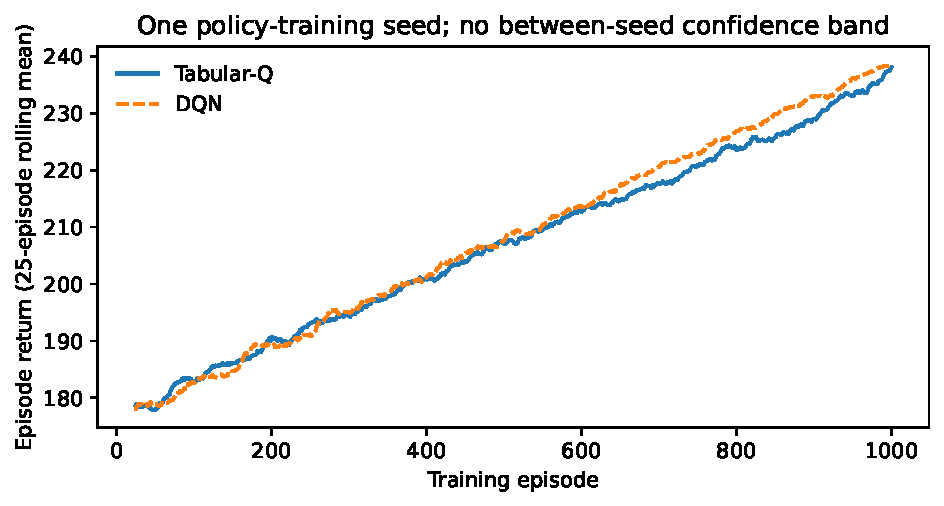
\includegraphics[width=.87\linewidth]{figures/training_returns.pdf}
\caption{Fixed-rate training returns. The trailing mean smooths the displayed curve only.}\label{fig:training}\end{figure}
\begin{figure}[h!]\centering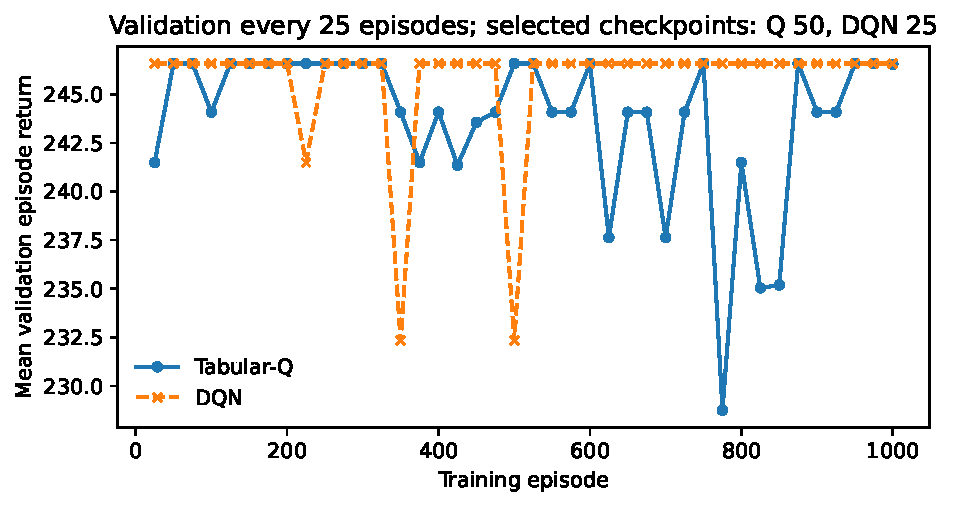
\includegraphics[width=.87\linewidth]{figures/validation_returns.pdf}
\caption{Fixed-rate validation returns and checkpoint selection. These checkpoints are separate from the final-episode policies in the main physical comparison.}\label{fig:validation}\end{figure}

Recorded process-start and artifact-creation timestamps delimit about 26.7 s for this Q run and 256.9 s for this DQN run. These are elapsed timestamp intervals from the fixed-rate training activity, not isolated training benchmarks and not timings for the 25 main-study policies. Training energy is not measured. The main comparison's training effort is reported as 500,000 recorded transitions per policy, with DQN replay updates configured after warm-up; it is performed offline and excluded from deployment energy.

A separate 324-state decision microbenchmark uses 30 blocks per state stream, each with 1,000 warm-up and 10,000 timed selections. On its observed-state stream, mean decision times are 0.739 microseconds for Static-LightLR, 6.582 microseconds for CFSM, 10.796 microseconds for Q, and 1.5669 ms for DQN. These timings characterize that implementation and state interface. They are not substituted for the current whole-device measurements or converted into controller-only energy.

\subsection{Reward and Hyperparameter Sensitivity}
The fixed-rate reward sweep includes seven Q configurations and four DQN configurations, each with five seeds (55 policies). All resource-aware configurations select LightLR on evaluated support; the five detection-only Q policies select MedRF. The thermal term is zero on the compact traces, so increasing its weight is not a test of thermal control. The following table reports the reward families only.
\begin{table}[h!]\centering\small
\caption{Fixed-rate reward sensitivity. LR counts LightLR-only policies; Single counts any single-action policy.}
\setlength{\tabcolsep}{3pt}
\begin{tabular}{lllrrrr}\toprule
Family & Algorithm & Variant & $n$ & LR & Single & Mean F1\\\midrule
\tableinput{tables/reward_rows}
\bottomrule\end{tabular}\end{table}

The associated state-removal experiment has five full-state controls, fifteen removals of constant temperature/queue/arrival coordinates, and ten removals of threat or previous-action coordinates. The fifteen constant-coordinate removals do not intervene on a varying signal and cannot establish adaptation to changes in those coordinates. They are not counted as fifteen independent robustness findings.

The fixed-rate Q hyperparameter sweep contains 35 policies. Its seven settings vary learning rate or discount while holding the remaining design fixed. All select LightLR throughout their evaluated support. These observations characterize that objective and support; they do not establish universal insensitivity to learning rate or discount.
\begin{table}[h!]\centering\small
\caption{Fixed-rate Q hyperparameter sensitivity. Each configuration has five seeds.}
\begin{tabular}{lrrrr}\toprule
Variant & $n$ & LR & Single & Mean F1\\\midrule
\tableinput{tables/hyperparameter_rows}
\bottomrule\end{tabular}\end{table}

\subsection{Finite-State Baseline}
The fixed-rate CFSM uses the recorded ordered detector pool, a 70$^\circ$C temperature warning, and threat threshold 0.7. Its exact transition priorities, one-step moves, two-window cooldown, and temperature override are given in the archived implementation. It is not one of the six methods in the main comparison, whose explicitly specified heuristic is DeadlineGuard. No fixed-rate CFSM measurement is pooled with that comparison.

\bibliographystyle{IEEEtran}\bibliography{references}
\end{document}
